\documentclass[a4paper,11pt]{article}
\usepackage[spanish]{babel} % Para escribir en Espa~nol normal
\usepackage[utf8]{inputenc}
%\usepackage[latin1]{inputenc}
\usepackage{color}
\usepackage{array}
\usepackage{amsmath,amssymb}
\usepackage{float}
\usepackage{graphicx}
\usepackage{subfig}
\begin{document}

%Portada del Documento
\setlength{\unitlength}{1 cm} %Especificar unidad de trabajo
\thispagestyle{empty}
\begin{picture}(18,3)
\put(4,0){
\includegraphics[width=4cm,height=5cm]{logo.jpg}}
\end{picture}
\begin{center}
\textbf{{\Huge Control de Gastos Personales}\\[0.5cm]
{\LARGE Proyecto del Primer Parcial }}\\[1.25cm]
{\Large Lenguajes de Programación}\\[2.3cm]
{\LARGE \textbf{Reporte}}\\[3.5cm]
\end{center}
{\Large Integrantes:}
\begin{itemize}
\item Vanessa Robles
\item Ricardo Campuzano
\item Ana Mora Ocaña
\end{itemize}
\begin{center}
 Ingeniería en Computación\\[0.3cm]
  ESPOL\\[1cm]
Guayaquil - \today
\end{center}
% fin de la portada

%%Tabla de Contenid
\newpage
\tableofcontents
\newpage
\section{ Problema a Resolver}

Actualmente,  hemos notado que a más de una persona que lleva una contabilidad para declarar sus impuestos en el SRI no sabe que hacer, esto se vuelve tormentoso a la hora de buscar facturas, saber cuanto gastos se ha realizado, recordar las fechas de declaración y por lo general las personas de poco conocimiento en el funcionamiento o manejo de esta entidad buscan contratar adicionalmente una persona que les realicen dicho proceso de llevar la contabilidad de sus actividades. Es este principal interés el que nos vemos en la necesidad de digitalizar dicha información de una manera màs facil para las personas natural que realizan esta actividad, la declaración de sus impuestos.

\section{ Descripción de la Aplicación}
Facture SRI esta diseñado para  personas naturales no obligadas a llevar contabilidad que deben cumplir con la presentación de la información relativa a los gastos personales deducidos por los constribuyentes para efecto de liquidación de Impuesto a la Renta.
Esta aplicación ayudará al usuario a llevar un mejor control de sus facturas, clasificando cada ingreso de datos de las facturas en el tipo de gasto que corresponda, asi como tambien generando un reporte detallado. 
El objetivo de la aplicación  es desarrollar una herramienta que permita a los ciudadanos comunes, llamados muchas veces  “ciudadanos de a pié”, generar de pago de impuestos sin la necesidad de utilizar el DIMM. La herramienta genera estos documentos a través del análisis de los gastos e ingresos del usuario previamente ingresados por el usuario.
Facture SRI  ayudará  recordando la fecha máxima de entrega de el reporte al SRI. 
Mediante la automatización el sistema clasificará la información por número de RUC del proveedor y tipo de gasto generando los siguientes reportes: 

\begin{figure} [h]
\begin {center}
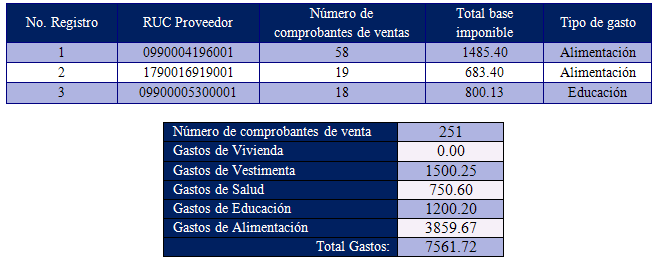
\includegraphics[width=1\textwidth]{img.png}
\end {center}
\end{figure}


\section{ Descripción del Contexto en Función de los Aspectos}
     \subsection{ Ambiente Físico}
En el entorno que será util la apliacación será según el lugar de encuentro del usuario en el momento de tener la factura en sus manos, porque de esta manera el usario no se olvidará de ingresar sus facturas ni perderlas.
En el momento que queremos enviar nuestro archivo generado al  SRI se deberá estar en un area donde tengamos disponibilidad al internet. Si la señal de internet es baja, puede que la aplicación presente problemas o simplemente no funcione.
Si en el entorno hay interferencia de señales externas como puede que se presenten errores en la transmisión de datos.
 La iluminación no sería un problema para el uso de nuestra aplicación debido a que la pantalla de los celulares tiene luz interna.
 Las condiciones de temperatura deben ser mayores a 0 grados centígrados, debido a que los requerimientos de seguridad de la mayoría de celulares sugieren usarlos a esta temperatura por las capacidades  de trabajo de la batería en el frío.
La mayoría de aplicaciones no están hechas para que puedan instalarse en una memoria micro SD, en realidad la gran mayoría por defecto se instalan en el espacio disponible de la memoria del teléfono por eso es frecuente que la memoria para instalarla nos resulte escasa.

    \subsection{ Ambiente Social}
Está aplicación esta dirigida  para personas naturales no obligadas a llevar contabilidad que deben cumplir que tienen problemas al momento de llevar el control de sus facturas para declaraciones de Gastos Personales en el SRI (Servicio de Rentas Internas).
La aplicación recordará al usuario las fechas que le toca hacer sus declaraciones al SRI según el informe que se ha generado al llevar la contabilidad de las facturas que se ha ido guardando. La aplicación también recordará las multas que tendría sino hace a tiempo sus declaraciones. 

   \subsection{ Ambiente Organizacional}
Nuestro ambiente organizacional está enfocado en el SRI y el usuario. El usuario es el que realiza la actividad de uso de la aplicación. También las personas CPA (Contador Público y Auditor) que llevan las contabilidad a personas para el SRI

El SRI no utiliza la aplicación pero es el que provee información de como debe estar estructurado el sistema.

   \subsection{ Ambiente Soporte de Usuario}
La aplicación consta de la opción “Ayuda” que tendrá la sección de “Preguntas frecuentes” con sus respectivas respuestas. En caso de que se presenten problemas, se mostrarán mensajes especificando el mismo.

    \subsection{ Restricciones}
\begin{itemize}
\item La aplicación será realizada en el idioma español.
\item La aplicación tiene solo uso para el Ecuador.
\item Los informes se generaran según los requisitos que indica el SRI, así como su valor y multas.
\end{itemize}

\section{ Prototipo de la Aplicación}
A continuación se muestran algunas imagenes de como podria llegar a quedar la aplicació, algunas pantallas podrian cambiar en el transcurso de implementación del proyecto.
El logo de la aplicacón es el siguiente:

\begin{figure} [h]
\begin {center}

\includegraphics[width=0.5\textwidth]{apli.png}
\end {center}
\end{figure}

    
\begin{figure}[ht!]
 \subsection{ Imagenes}
   \centering
   %%----primera subfigura----
   \subfloat[]{
        \label{fig:pantalla:1}         %% Etiqueta para la primera subfigura
        
\includegraphics[width=0.42\textwidth]{img1.png}}
   \hspace{0.1\linewidth}
   %%----segunda subfigura----
   \subfloat[]{
        \label{fig:pantalla:2}         %% Etiqueta para la segunda subfigura
        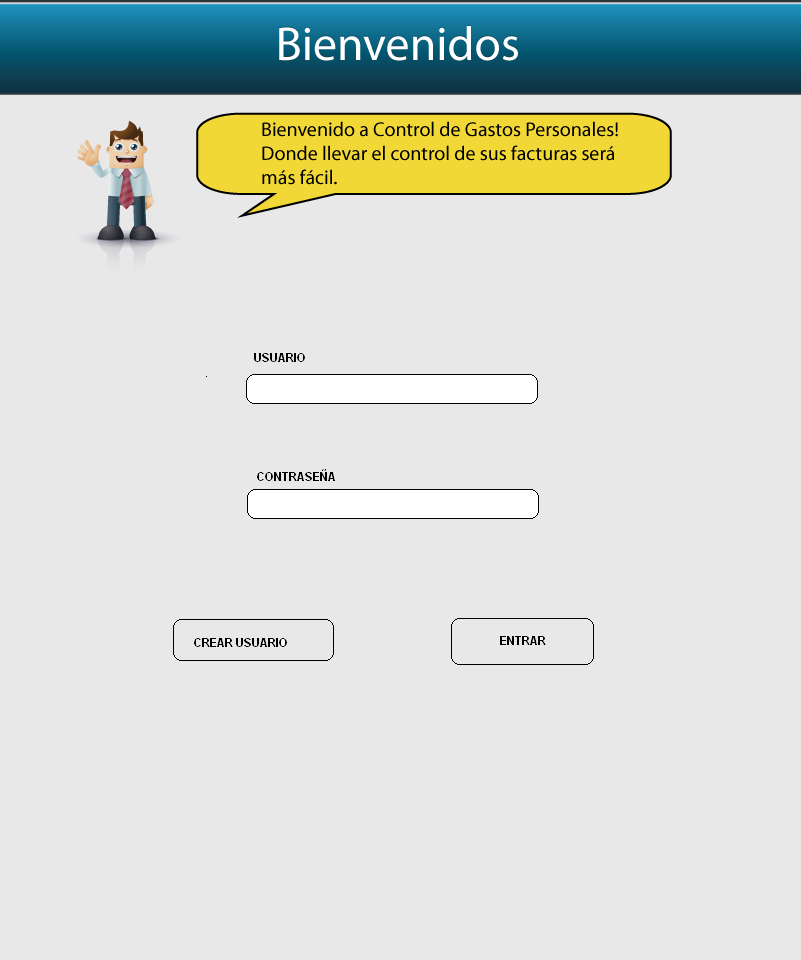
\includegraphics[width=0.42\textwidth]{img2.png}}\\[20pt]
   %%----tercera subfigura----
   \subfloat[]{
        \label{fig:pantalla:3}         %% Etiqueta para la tercera subfigura
        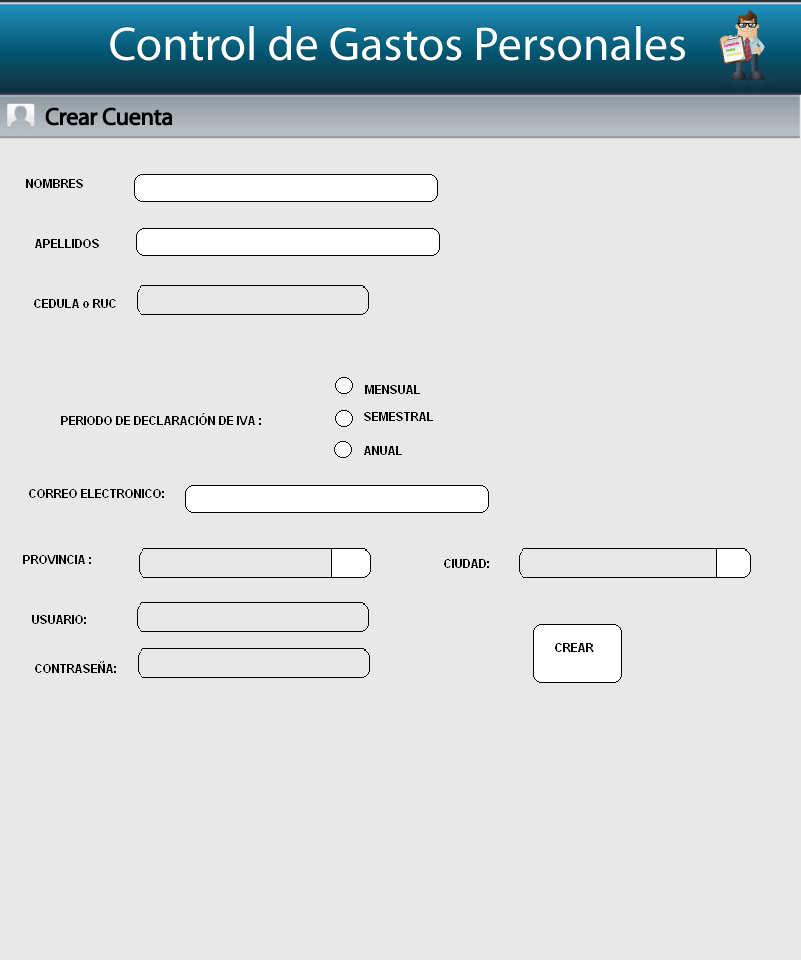
\includegraphics[width=0.42\textwidth]{img3.png}}
    \hspace{0.1\linewidth}
   %%----cuarta subfigura----
    \subfloat[]{
        \label{fig:pantalla:4}         %% Etiqueta para la cuarta subfigura
        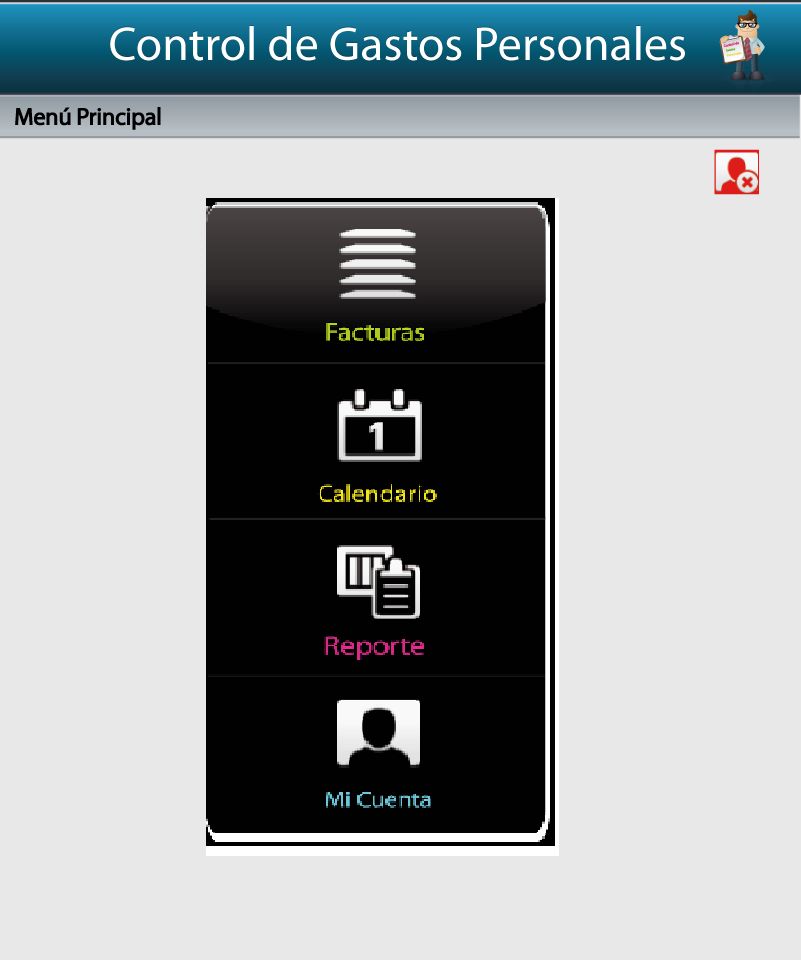
\includegraphics[width=0.42\textwidth]{img4.png}}
\hspace{0.1\linewidth}
 %%----quinta subfigura----
   \subfloat[]{
        \label{fig:pantalla:5}         %% Etiqueta para la tercera subfigura
        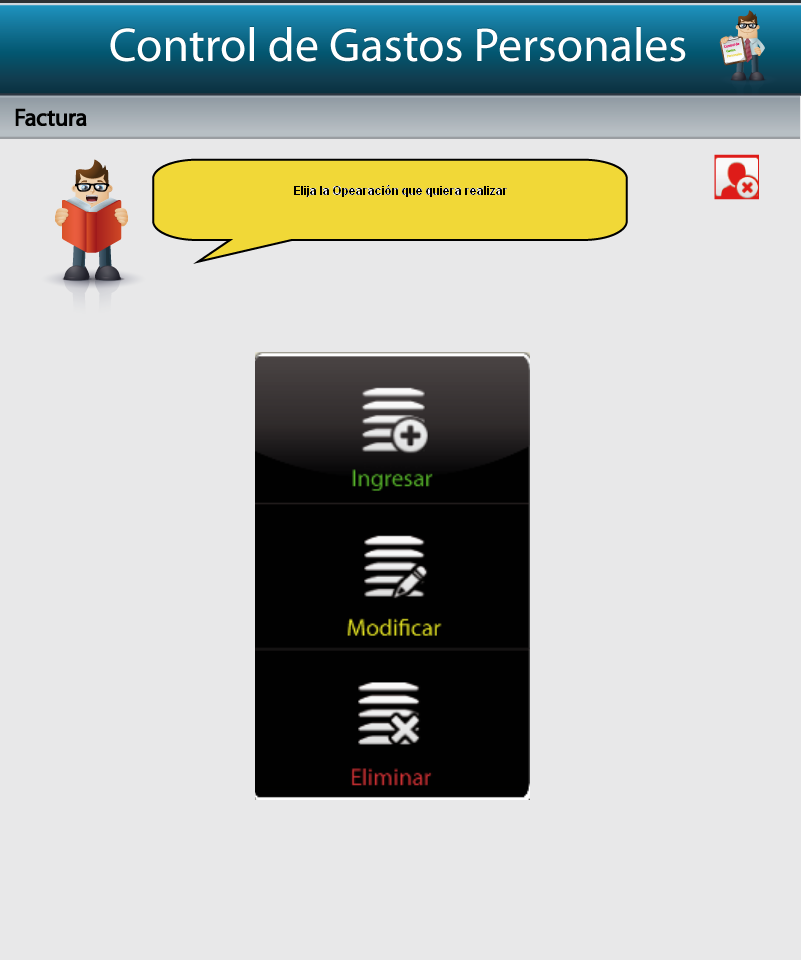
\includegraphics[width=0.42\textwidth]{img5.png}}
\hspace{0.1\linewidth}
%%----sexta subfigura----
   \subfloat[]{
        \label{fig:pantalla:6}         %% Etiqueta para la tercera subfigura
        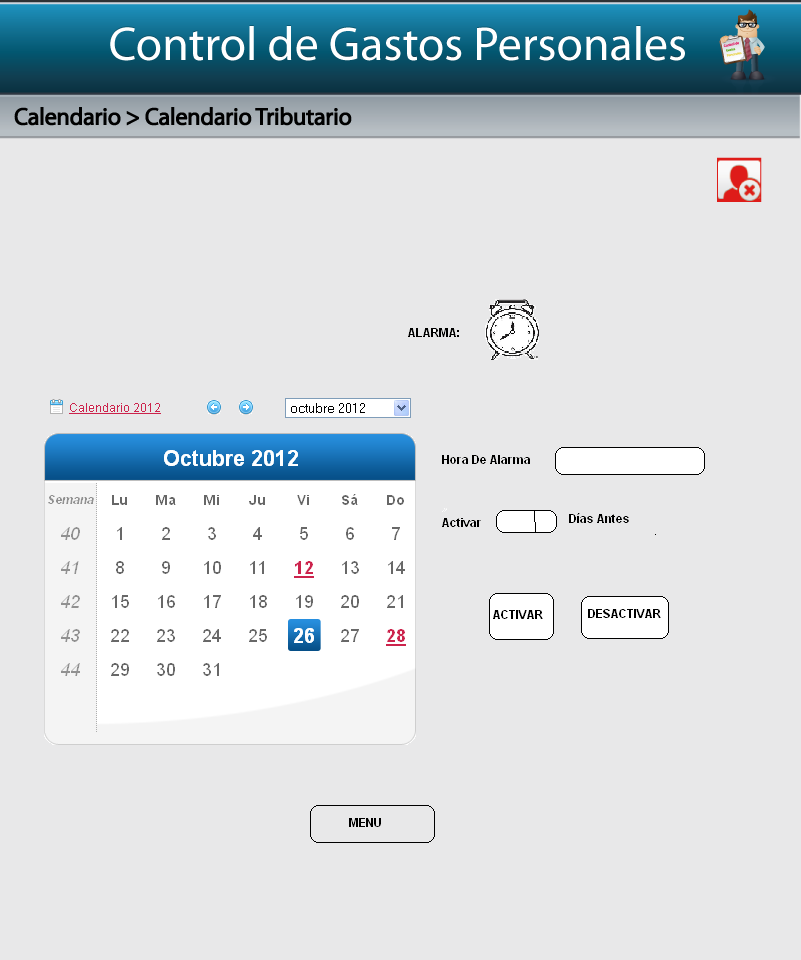
\includegraphics[width=0.42\textwidth]{img6.png}}

  

\end{figure}


\end {document}

